% -*- root: main.tex -*-
%-------------------------------------------------------------------------------
\chapterimage{chapter_head_7.pdf} 

%-------------------------------------------------------------------------------
\chapter{ROS 기본 프로그래밍}

%-------------------------------------------------------------------------------
\section{메시지, 토픽, 서비스, 매개변수}\index{메시지, 토픽, 서비스, 매개변수}

%-------------------------------------------------------------------------------
\subsection{ROS 메시지 통신}\index{ROS 메시지 통신}

다음 강좌부터 ROS 프로그래밍이 시작된다. 이전 강좌들이 개론을 설명하였다면 이번 부터가 본격적인 ROS 강좌라고 볼 수 있다. 하지만, 이전 강좌들도 필수적으로 알아야할 기초이므로 꼭 정독하시기를 권장한다. 특히, 이번 강좌를 따라오기 위해서는 아래의 강좌는 필수 사항이라고 볼 수 있다.\\

로봇 운영체제 강좌 : 08. ROS 용어 정리\\
로봇 운영체제 강좌 : 09. ROS 개념 정리\\

지금까지 다양한 강좌들을 올렸는데, 제일 많이 나온 단어라고 치면 "메시지, 토픽, 서비스, 매개변수" 가 가장 빈번히 언급되었다. 그도 그럴것이, 메시지, 토픽, 서비스, 매개변수는 ROS 에서 가장 핵심 부분이라고 할 수 있다. 각기 목적에 따라 분화된 최소 실행 단위인 노드들은 메시지 통신을 통해 노드간의 입/출력 데이터를 주고 받는 처리를 하고 있다.

\begin{definition*}[메시지(message,msg)]
노드는 메시지를 통해 노드간의 데이터를 주고받게 된다. 메시지는 integer, floating point, boolean 와 같은 변수형태이다. 또한, 메시지안에 메시지를 품고 있는 간단한 데이터 구조 및 메시지들의 배열과 같은 구조도 사용할 수 있다. 

메세지를 이용한 통신방법으로는 TCPROS, UDPROS 방식등이 있으며, 단방향 메시지 송/수신 방식의 토픽과 양방향 메시지 요청/응답 방식의 서비스를 이용하고 있다.
\end{definition*}

메시지 통신을 하나의 그림으로 설명하면 아래와 같다고 볼 수 있다. 작은 목적 단위로 세분화된 실제 처리 프로그램인 노드는 다른 노드와의 데이터 송수신에 메시지 통신 방법을 이용하고 있다. 이 메시지 통신에는 크게 토픽과 서비스로 나뉘고 큰 틀에서는 매개변수 또한 메시지 통신이라고 볼 수있다. 이 세가지 메시지 통신방식인 토픽, 서비스, 매개변수를 이번 강좌에서 소개하고 각각의 특징을 ROS 프로그램 작성전에 미리 익혀두고자 한다. 그 후, 이어지는 강좌들에서 실전을 통해 자세히 다룰 예정이다.

\begin{figure}[h]
\centering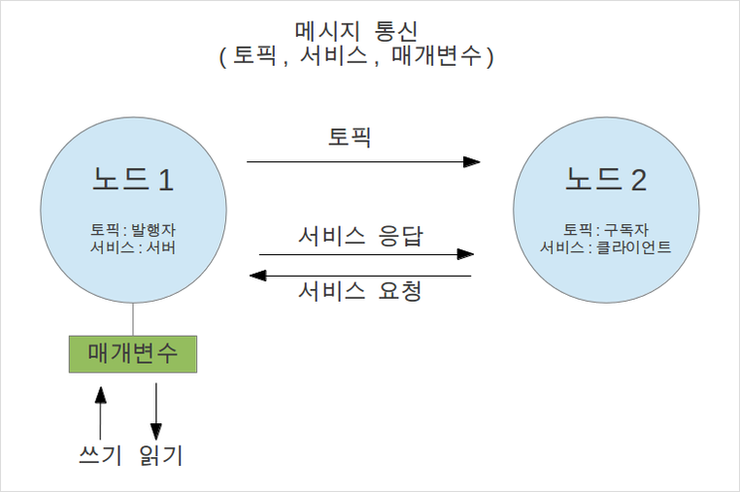
\includegraphics[width=0.5\columnwidth]{pictures/chapter7/msgtrans1.png}
\caption{메시지 통신 상관 관계}
\end{figure}

%-------------------------------------------------------------------------------
\subsection{토픽 (topic)}\index{토픽 (topic)}

토픽(topic)은 "이야깃거리"이다.\\ 

발행자 노드가 하나의 이야깃거리에서 대해서 토픽이라는 이름으로 마스터에 등록한 후, 이야깃거리에 대한 이야기를 메시지 형태로 발행한다. 이 이야깃거리를 수신 받기를 원하는 구독자 노드는 마스터에 등록된 토픽의 이름에 해당되는 발행자 노드의 정보를 받는다. 이 정보를 기반으로 구독자 노드는 발행자 노드와 직접적으로 연결하여 메시지를 송/수신 받게 된다. \\

이를 나타낸 그림이 아래와 같다. 단방향 통신이기에 센서가 취득한 정보를 단순히 전달하는 용도로 많이 사용되는 메시지 통신 방식이다.

\begin{figure}[h]
\centering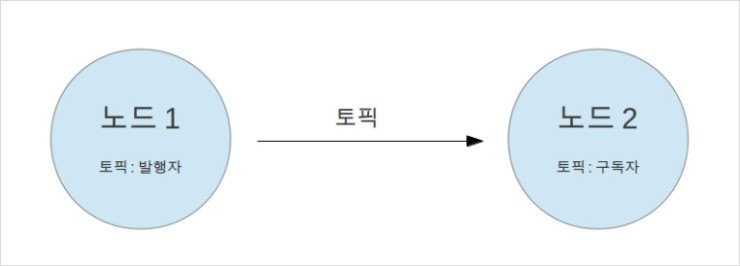
\includegraphics[width=0.5\columnwidth]{pictures/chapter7/msgtrans2.jpg}
\caption{토픽}
\end{figure}

%-------------------------------------------------------------------------------
\subsection{서비스(service)}\index{서비스(service)}

발행과 구독 개념의 토픽 통신 방식은 비동기 방식이라 필요에 따라서 주어진 데이터를 전송하고 받기에 매우 훌륭한 방법이다. 또한, 한번의 접속으로 지속적인 메시지를 송/수신하기 때문에 지속적으로 메시지를 발송해야하는 센서 데이터에 적합하여 많이 사용되고 있다. 

하지만, 경우에 따라서는 요청과 응답이 함께 사용되는 동기 방식의 메시지 교환 방식도 필요하다. 이에 따라, ROS에서는 서비스라는 이름으로 메시지 동기 방식을 제공하고 있다. 

서비스는 요청이 있을 경우에 응답을 하는 서비스 서버와 요청을 하고 응답을 받는 서비스 클라이언트로 나뉘어 있다. 서비스는 토픽과는 달리 1회성 메시지 통신이다. 서비스의 요청과 응답이 완료되면 연결된 두 노드의 접속은 끊기게 된다. 

이러한 서비스는 로봇에게 특정의 일을 수행하는 요청시에 명령어로써 많이 사용된다. 혹은, 특정 조건에 의해 이벤트를 발생해야할 노드에 사용되는 경우가 많다. 1회성 메시지 이기에 네트워크에 부하가 적다는 이유로 토픽을 대체하는 수단으로도 사용되는 등 매우 유용한 통신 수단이다.

\begin{figure}[h]
\centering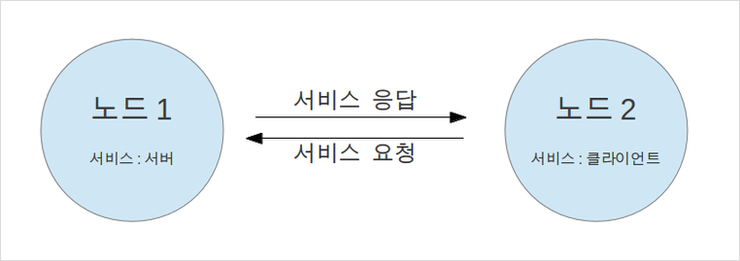
\includegraphics[width=0.5\columnwidth]{pictures/chapter7/msgtrans3.png}
\caption{서비스}
\end{figure}

%-------------------------------------------------------------------------------
\subsection{매개변수(parameter)}\index{매개변수(parameter)}

노드에서 사용되는 매개변수를 말한다. 흔히, 윈도우즈 프로그램에서 *.ini 설정파일과 같다고 생각하면 된다. 디폴트로 설정 값들이 지정되어 있고, 필요에 의해서 외부에서 이 매개변수를 읽기, 쓰기가 가능하다. 특히, 상황에 맞추어 이 매개변수를 외부에서 쓰기기능을 이용하여 설정값을 실시간으로 바꿀수 있기에 매우 유용한 방법이다. 이는 엄밀히 따지면, 메시지 통신이라고 볼 수 없지만, 필자는 메시지를 이용한다는 점에서 메시지 통신의 범위에 속한다고 본다. 사용 예를 들자면 접속하는 USB포트 및 카메라 캘리브레이션 값, 속도 및 명령어들의 최대/최저 값 등의 설정 등을 꼽을 수 있다.

\begin{figure}[h]
\centering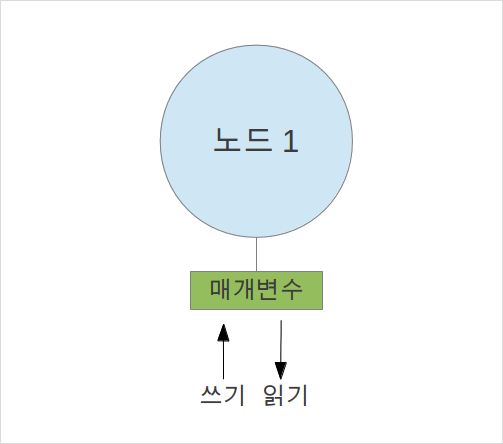
\includegraphics[width=0.5\columnwidth]{pictures/chapter7/msgtrans4.png}
\caption{매개변수}
\end{figure}

%-------------------------------------------------------------------------------
\section{메시지 발행자 노드와 구독자 노드 작성 및 실행}\index{메시지 발행자 노드와 구독자 노드 작성 및 실행}

%-------------------------------------------------------------------------------
\subsection{목적}

ROS 메시지 통신에서 사용되는 발행자(Publisher) 와 구독자(Subscriber) 라는 용어는 쉽게 우리말로 따지면 송신과 수신역할을 담당하게 된다. ROS에서는 송신측을 Publisher, 수신측을 Subscriber 라고 부르고 있다. 이 강좌에서는 간단한 메시지 파일을 작성해보고, 발행자(Publisher) 노드 와 구독자(Subscriber) 노드를 작성 및 실행하는 것을 목적으로 한다.

이 강좌를 수행하기 앞서서 참고가 될만한 선행 강좌를 아래에 링크한다. 메시지 통신, 토픽, cakin 빌드 시스템, 패키지, 노드 등의 용어를 잘 모르겠다면 아래의 강좌를 참조하길 바란다.\\

로봇 운영체제 강좌 : 08. ROS 용어 정리\\
로봇 운영체제 강좌 : 09. ROS 개념 정리\\
로봇 운영체제 강좌 : 11. ROS 빌드 시스템\\
로봇 운영체제 강좌 : 14. 메시지, 토픽, 서비스, 매개변수\\

%-------------------------------------------------------------------------------
\subsection{패키지 생성}

아래의 명령어는 "oroca\_ros\_tutorials" 라는 패키지를 생성하는 명령어이다. 이 패키지는 의존하는 패키지로 "std\_msgs"와 "roscpp"를 옵션으로 달아주었다. 로스의 표준 메시지 패키지인 std\_msgs 와 로스에서 c/c++을 사용하기 위하여 클라이언트라이브러인 roscpp를 사용하겠다는 것으로 패키지 생성에 앞어서 미리 설치해야한다는 의미이다. 이러한 의존하는 패키지의 설정은 패키지 생성할 때 지정할 수도 있지만, 생성 후 package.xml 에서 직접 입력하여도 된다.

\begin{lstlisting}[language=ROS]
$ cd ~/catkin_ws/src
$ catkin_create_pkg oroca_ros_tutorials std_msgs roscpp
\end{lstlisting}

위와 같이 패키지를 생성하였으면 "~/catkin\_ws/src"에 "oroca\_ros\_tutorials" 라는 패키지 폴더 및 ROS 패키지가 갖추어야할 기본 내부 폴더 및 CMakeLists.txt 와 package.xml가 생성된다. 다음은 아래와 같이 ls 명령어를 입력하여 내용을 보던가 윈도우의 탐색기와 같은 역할을 하는 GUI기반의 Nautilus를 이용하여 패키지 내부를 살펴보도록 하자.

\begin{lstlisting}[language=bash]
$ ls
include       %*.......... 인클루드 폴더*)
src           %*.......... 소스코드 폴더*)
CMakeLists.txt%*.......... 빌드 설정 파일*)
\end{lstlisting}

%-------------------------------------------------------------------------------
\subsection{패키지 설정 파일 (package.xml) 수정}

ROS의 필수 설정 파일 중 하나인 package.xml 은 패키지 정보를 담은 XML 파일로써 패키지의 이름, 저작자, 라이선스, 의존성 패키지 등을 기술하고 있다. 아래의 명령어로 gedit 툴을 이용하여 파일을 열고 현재의 노드에 맞도록 수정해보자.

\begin{lstlisting}[language=bash]
$ gedit package.xml 
\end{lstlisting}

아래의 코드는 package.xml 를 이번 노드에 맞도록 수정한 내용이다. 내용중에 필자의 개인 정보가 포함되어 있으니, 이를 자신에 맞게 수정해주길 바란다. 각 옵션의 세부 설명은 로봇 운영체제 강좌 : 11. ROS 빌드 시스템 를 참고하길 바란다.

\begin{lstlisting}[language=XML]
<?xml version="1.0"?>
<package>
  <name>oroca_ros_tutorials</name>
  <version>0.1.0</version>
  <description>The oroca_ros_tutorials package</description>

  <maintainer email="passionvirus@gmail.com">Yoonseok Pyo</maintainer>
  <url type="website">http://oroca.org</url>
  <url type="repository">https://github.com/oroca/oroca_ros_tutorials.git</url>
  <author email="passionvirus@gmail.com">Yoonseok Pyo</author>

  <license>MIT</license>

  <buildtool_depend>catkin</buildtool_depend>

  <build_depend>roscpp</build_depend>
  <build_depend>std_msgs</build_depend>
  <build_depend>message_generation</build_depend>

  <run_depend>roscpp</run_depend>
  <run_depend>std_msgs</run_depend>
  <run_depend>message_runtime</run_depend>

  <export>
  </export>
</package>
\end{lstlisting}

%-------------------------------------------------------------------------------
\subsection{빌드 설정 파일 (CMakeLists.txt) 수정}

ROS의 빌드 시스템인 캐킨(cakin)은 기본적으로 CMake를 이용하고 있어서 패키지 폴더에 CMakeLists.txt 라는 파일에 빌드 환경을 기술하고 있다. 이는 실행 파일 생성, 의존성 패키지 우선 빌드, 링크 생성 등을 설정하게 되어 있다.

\begin{lstlisting}[language=bash]
$ gedit CMakeLists.txt 
\end{lstlisting}

아래의 코드는 CMakeLists.txt 를 이번 노드에 맞도록 수정한 내용이다. 각 옵션의 세부 설명은 로봇 운영체제 강좌 : 11. ROS 빌드 시스템 를 참고하길 바란다.

\begin{lstlisting}[language=make]
cmake_minimum_required(VERSION 2.8.3)
project(oroca_ros_tutorials)

## Find catkin and any catkin packages
find_package(catkin REQUIRED COMPONENTS roscpp std_msgs message_generation)

## Declare ROS messages and services
add_message_files(FILES msgTutorial.msg)

## Generate added messages and services
generate_messages(DEPENDENCIES std_msgs)

## Declare a catkin package
catkin_package(
  #INCLUDE_DIRS include
  LIBRARIES oroca_ros_tutorials
  CATKIN_DEPENDS roscpp std_msgs
  DEPENDS system_lib
)

## Build node
include_directories(include ${catkin_INCLUDE_DIRS})

add_executable(ros_tutorial_msg_publisher src/ros_tutorial_msg_publisher.cpp)
target_link_libraries(ros_tutorial_msg_publisher ${catkin_LIBRARIES})
add_dependencies(ros_tutorial_msg_publisher oroca_ros_tutorials_generate_messages_cpp)

add_executable(ros_tutorial_msg_subscriber src/ros_tutorial_msg_subscriber.cpp)
target_link_libraries(ros_tutorial_msg_subscriber ${catkin_LIBRARIES})
add_dependencies(ros_tutorial_msg_subscriber oroca_ros_tutorials_generate_messages_cpp)
\end{lstlisting}

%-------------------------------------------------------------------------------
\subsection{메시지 파일 작성}

CMakeLists.txt 에 라는 파일에 "add\_message\_files(FILES msgTutorial.msg)" 라는 옵션을 넣었다. 이는 이번 노드에서 사용할 메시지인 msgTutorial.msg 를 빌드할때 포함하라는 이야기이다. 현재, msgTutorial.msg 는 생성하지 않았기에 아래와 같은 순서로 생성해주도록 하자.

\begin{lstlisting}[language=bash]
$ cd ~/catkin_ws/src/oroca_ros_tutorials/     %*(패키지 폴더로 이동한다.)*)
$ mkdir msg               %*(패키지에 msg 라는 메시지 폴더를 신규 작성한다.)*)
$ cd msg                  %*(작성한 msg 폴더로 이동)*)
$ gedit msgTutorial.msg   %*(msgTutorial.msg 파일 신규 작성 및 내용 수정)*)
\end{lstlisting}

내용으로는 아래와 같이 int32 메시지 형식에 data라는 이름의 메시지를 만들어주자.

\begin{lstlisting}[language=ROS]
int32 data
\end{lstlisting}

%-------------------------------------------------------------------------------
\subsection{발행자 노드 작성}

\begin{lstlisting}[language=make]
add_executable(ros_tutorial_msg_publisher src/ros_tutorial_msg_publisher.cpp)
\end{lstlisting}

CMakeLists.txt 에 위와 같은 실행 파일을 생성하는 옵션을 주었다. 즉, "ros\_tutorial\_msg\_publisher.cpp"라는 파일을 빌드하여 "ros\_tutorial\_msg\_publisher"라는 실행 파일을 만들라는 이야기이다. 아래의 순서대로 발행자 노드 기능을 수행하는 "ros\_tutorial\_msg\_publisher.cpp" 소스를 작성해 보자. 

\begin{lstlisting}[language=bash]
$ cd ~/catkin_ws/src/oroca_ros_tutorials/ %*(패키지 폴더로 이동한다.)*)
$ cd src                                  %*(노드의 소스코드 폴더인 src 폴더로 이동)*)
$ gedit ros_tutorial_msg_publisher.cpp    %*(소스 파일 신규 작성 및 내용 수정)*)
\end{lstlisting}

\begin{lstlisting}[language=C++]
#include "ros/ros.h"                         //%* ROS 기본 헤더파일*)
#include "oroca_ros_tutorials/msgTutorial.h" //%* msgTutorial 메시지 파일헤더*)

int main(int argc, char **argv)              //%* 노드 메인 함수*)
{
  ros::init(argc, argv, "ros_tutorial_msg_publisher");  //%* 노드명 초기화*)
  ros::NodeHandle nh;                                   //%* 노드 핸들 선언*)

  //%* 발행자 선언, oroca\_ros\_tutorials 패키지의 msgTutorial 메시지 파일을 이용한*)
  //%* 발행자 ros\_tutorial\_pub 를 작성한다. 토픽명은 "ros\_tutorial\_msg" 이며,*)
  //%* 발행자 큐(queue) 사이즈를 100개로 설정한다는 것이다*)
  ros::Publisher ros_tutorial_pub = nh.advertise<oroca_ros_tutorials::msgTutorial>("ros_tutorial_msg", 100);

  //%* 루프 주기를 설정한다. "10" 이라는 것은 10Hz를 말하는 것으로 0.1초 간격으로 반복된다*)
  ros::Rate loop_rate(10); 

  int count = 0;    //%* 메시지에 사용될 변수 선언*)

  while (ros::ok())
  {
    oroca_ros_tutorials::msgTutorial msg; //%* msgTutorial 형식으로 msg 메시지를 선언*)
    msg.data = count;                 //%* count 변수를 이용하여 메시지 값을 정한다*)

    ROS_INFO("send msg = %d", count); //%* ROS\_INFO 함수를 이용하여 count 변수 표시*)

    ros_tutorial_pub.publish(msg);    //%* 메시지를 발행한다. 약 0.1초 간격으로 발행된다*)

    loop_rate.sleep();                //%* 위에서 정한 루프 주기에 따라 슬립에 들어간다*)

    ++count;                          //%* count 변수 1씩 증가*)
  }

  return 0;
}
\end{lstlisting}

%-------------------------------------------------------------------------------
\subsection{구독자 노드 작성}

\begin{lstlisting}[language=make]
add_executable(ros_tutorial_msg_subscriber src/ros_tutorial_msg_subscriber.cpp)
\end{lstlisting}

CMakeLists.txt 에 위와 같은 실행 파일을 생성하는 옵션을 주었다. 즉, "ros\_tutorial\_msg\_subscriber.cpp"라는 파일을 빌드하여 "ros\_tutorial\_msg\_subscriber"라는 실행 파일을 만들라는 이야기이다. 아래의 순서대로 구독자 노드 기능을 수행하는 "ros\_tutorial\_msg\_subscriber.cpp" 소스를 작성해 보자. 

\begin{lstlisting}[language=bash]
$ cd ~/catkin_ws/src/oroca_ros_tutorials/ %*(패키지 폴더로 이동한다.)*)
$ cd src                                  %*(노드의 소스코드 폴더인 src 폴더로 이동)*)
$ gedit ros_tutorial_msg_subscriber.cpp   %*(소스 파일 신규 작성 및 내용 수정)*)
\end{lstlisting}

\begin{lstlisting}[language=C++]
#include "ros/ros.h"                         //%* ROS 기본 헤더파일*) 
#include "oroca_ros_tutorials/msgTutorial.h" //%* msgTutorial 메시지 파일 헤더*)

//%* 메시지 콜백함수로써, 밑에서 설정한 ros\_tutorial\_sub 구독자에 해당되는 메시지를*)
//%* 수신하였을때 동작하는 함수이다*)
//%* 입력 메시지로는 oroca\_ros\_tutorial 패키지의 msgTutorial 메시지를 받도록 되어있다 *)
void msgCallback(const oroca_ros_tutorials::msgTutorial::ConstPtr& msg)
{
  ROS_INFO("recieve msg: %d", msg->data);   //%* 수신된 메시지를 표시하는 함수*)
}

int main(int argc, char **argv)                         //%* 노드 메인 함수*)
{
  ros::init(argc, argv, "ros_tutorial_msg_subscriber"); //%* 노드명 초기화*)

  ros::NodeHandle nh;                                   //%* 노드 핸들 선언*)

  //%* 구독자 선언, oroca\_ros\_tutorials 패키지의 msgTutorial 메시지 파일을 이용한*)
  //%* 구독자 ros\_tutorial\_sub 를 작성한다. 토픽명은 "ros\_tutorial\_msg" 이며,*)
  //%* 구독자 큐(queue) 사이즈를 10개로 설정한다는 것이다*)
  ros::Subscriber ros_tutorial_sub = nh.subscribe("ros_tutorial_msg", 10, msgCallback);

  //%* 콜백함수 호출을 위한 함수로써, 메시지가 수신되기를 대기, 수신되었을 경우 콜백함수를 실행한다*)
  ros::spin();

  return 0;
}
\end{lstlisting}

%-------------------------------------------------------------------------------
\subsection{ROS 노드 빌드}

\begin{lstlisting}[language=bash]
$ cd ~/catkin_ws  %*(catkin 폴더로 이동)*)
$ catkin_make     %*(catkin 빌드 실행)*)
\end{lstlisting}

위의 명령어로 oroca\_ros\_tutorials 패키지의 메지시 파일, 발행자 노드, 구독자 노드가 빌드되었다. 
oroca\_ros\_tutorials 패키지의 소스는 ~/catkin\_ws/src/oroca\_ros\_tutorials/src 에 존재하고,oroca\_ros\_tutorials 패키지의 메시지 파일은 ~/catkin\_ws/src/oroca\_ros\_tutorials/msg 에 존재한다.

이를 기반으로 빌드된 결과물은 ~/catkin\_ws 의 /build 및 /devel 에 각각 생성된다.
/build 에는 캐킨 빌드에서 사용된 설정 내용이 저장되며, /devel/lib/oroca\_ros\_tutorials 에는 실행 파일이, /devel/include/oroca\_ros\_tutorials 에는 메시지 파일로부터 자동 생성된 메시지 헤더파일이 저장된다. 각 생성 결과물이 궁금하다면 이 경로에 생성된 결과물을 확인해 보자.

%-------------------------------------------------------------------------------
\subsection{발행자 실행}

※ 주의! 노드 실행에 앞서서 roscore를 실행해주는 것을 잊지 말자!

\begin{lstlisting}[language=ROS]
$ rosrun oroca_ros_tutorials ros_tutorial_msg_publisher
\end{lstlisting}

ROS 노드 실행 명령어인 rosrun 을 이용하여, oroca\_ros\_tutorials 패키지의 ros\_tutorial\_msg\_publisher 노드를 구동하라는 명령어이다. 이를 실행하게 되면 아래와 같은 출력 화면을 볼 수 있다. 내부에 선언된 count 값이 표시되고 있으며, ROS 메시지로 발부되고 있다. 

\begin{figure}[h]
\centering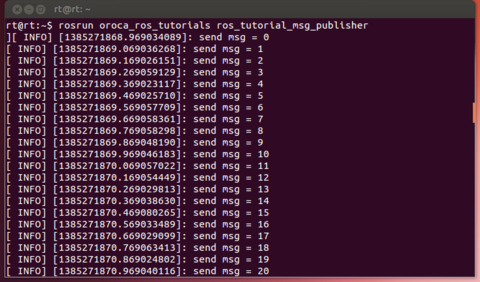
\includegraphics[width=0.5\columnwidth]{pictures/chapter7/rosrun_ros_tutorial_msg_publisher.png}
\caption{ros\_tutorial\_msg\_publisher 노드 실행시의 화면}
\end{figure}

이전에 익힌 rostopic 명령어를 이용하여 현재 ROS 네트워크에서 사용중인 토픽의 목록을 확인해보고, 위에서 실행한 발행자 노드에서 발행중인 메시지를 확인해보도록 하자.

\begin{lstlisting}[language=ROS]
$ rostopic list
/ros_tutorial_msg
/rosout
/rosout_agg
$ rostopic echo /ros_tutorial_msg
\end{lstlisting}

rostopic list 라는 옵션을 붙인 명령어로 "ros\_tutorial\_msg" 토픽이 있음을 확인하였다. rostopic echo /ros\_tutorial\_msg 이라는 명령어로 "ros\_tutorial\_msg" 토픽의 메시지를 확인해보자. 아래와 같이 실시간으로 발행되는 메시지를 확인할 수 있을 것이다.

\begin{figure}[h]
\centering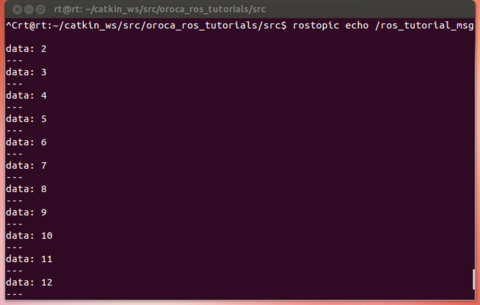
\includegraphics[width=0.5\columnwidth]{pictures/chapter7/rostopic_echo.png}
\caption{ros\_tutorial\_msg 토픽의 수신된 내역}
\end{figure}

%-------------------------------------------------------------------------------
\subsection{구독자 실행}

\begin{lstlisting}[language=ROS]
$ rosrun oroca_ros_tutorials ros_tutorial_msg_subscriber 
\end{lstlisting}

ROS 노드 실행 명령어인 rosrun 을 이용하여, oroca\_ros\_tutorials 패키지의 ros\_tutorial\_msg\_subscriber  노드를 구동하라는 명령어이다. 이를 실행하게 되면 아래와 같은 출력 화면을 볼 수 있다. 발행자에서 발행된 "ros\_tutorial\_msg" 토픽의 메시지를 수신받아 값이 표시되고 있다.

\begin{figure}[h]
\centering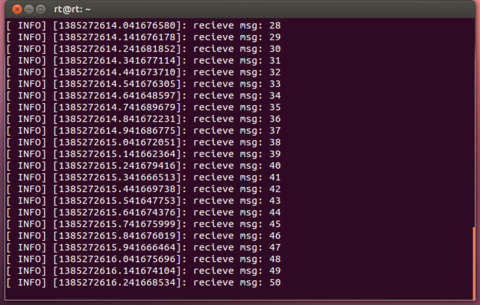
\includegraphics[width=0.5\columnwidth]{pictures/chapter7/rosrun_ros_tutorial_msg_subscriber.png}
\caption{ros\_tutorial\_msg\_subscriber 노드 실행시의 화면}
\end{figure}

%-------------------------------------------------------------------------------
\subsection{실행된 노드들의 통신 상태 확인}

\begin{lstlisting}[language=ROS]
$ rqt_graph
\end{lstlisting}
또는

\begin{lstlisting}[language=ROS]
$ rqt
\end{lstlisting}

rqt 를 실행 후, 플러그인(plugins)에서 ROS Graph 를 선택하면 아래의 그림처럼 현재 ROS 에서 구동중인 노드 및 메시지를 확인할 수 있다. 현재 ROS 네트워크상에는, 구독자 노드 (ros\_tutorial\_msg\_publisher) 에서 발행한 토픽 (ros\_tutorial\_msg) 이 발행중이고 이를 구독자 노드 (ros\_tutorial\_msg\_subscriber) 에서 수신하고 있음을 확인할 수 있다.

\begin{figure}[h]
\centering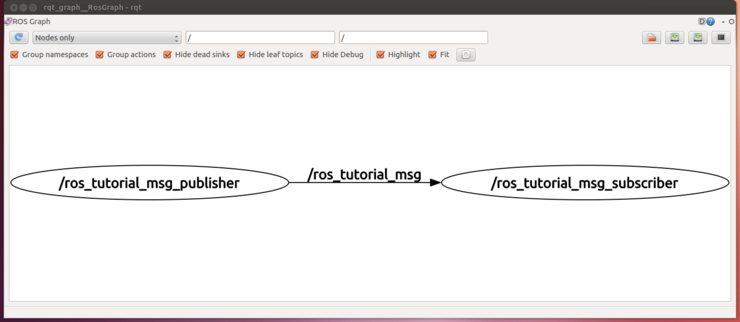
\includegraphics[width=0.5\columnwidth]{pictures/chapter7/rqt_graph_oroca_ros_tutorials.png}
\caption{rqt\_graph를 통해서 본 두 노드의 관계도}
\end{figure}

%-------------------------------------------------------------------------------
\section{서비스 서버 노드와 클라이언트 노드 작성 및 실행}\index{서비스 서버 노드와 클라이언트 노드 작성 및 실행}

%-------------------------------------------------------------------------------
\subsection{서비스의 목적}

서비스는 요청이 있을 경우에 응답을 하는 서비스 서버와 요청을 하고 응답을 받는 서비스 클라이언트로 나뉘어 있다. 서비스는 토픽과는 달리 1회성 메시지 통신이다. 서비스의 요청과 응답이 완료되면 연결된 두 노드의 접속은 끊기게 된다.이러한 서비스는 로봇에게 특정의 일을 수행하는 요청시에 명령어로써 많이 사용된다. 혹은, 특정 조건에 의해 이벤트를 발생해야할 노드에 사용되는 경우가 많다. 1회성 메시지 이기에 네트워크에 부하가 적다는 이유로 토픽을 대체하는 수단으로도 사용되는 등 매우 유용한 통신 수단이다.

이 강좌에서는 간단한 서비스 파일 작성해보고 서비스 서버(server) 노드 와 서비스 클라이언트(client) 노드를 작성 및 실행하는 것을 목적으로 한다.

이 강좌를 수행하기 앞서서 참고가 될만한 선행 강좌를 아래에 링크한다. 메시지 통신, 서비스, cakin 빌드 시스템, 패키지, 노드 등의 용어를 잘 모르겠다면 아래의 강좌를 참조하길 바란다.\\

로봇 운영체제 강좌 : 08. ROS 용어 정리\\
로봇 운영체제 강좌 : 09. ROS 개념 정리\\
로봇 운영체제 강좌 : 11. ROS 빌드 시스템\\
로봇 운영체제 강좌 : 14. 메시지, 토픽, 서비스, 매개변수\\

%-------------------------------------------------------------------------------
\subsection{패키지 생성}

이전 강좌에서 "oroca\_ros\_tutorials" 라는 패키지를 생성하는 설명을 하였다. 위 강좌를 참조하기 바라고, 위 강좌에서 이미 패키지를 생성한 것으로 보고 패키지 생성은 건너 뛰도록 하자.

%-------------------------------------------------------------------------------
\subsection{패키지 설정 파일 (package.xml) 수정}

이번 강좌에서는 패키지 정보를 담은 package.xml 를 수정할 부분이 없다.

%-------------------------------------------------------------------------------
\subsection{빌드 설정 파일 (CMakeLists.txt) 수정}

ROS의 빌드 시스템인 캐킨(cakin)은 기본적으로 CMake를 이용하고 있어서 패키지 폴더에 CMakeLists.txt 라는 파일에 빌드 환경을 기술하고 있다. 이는 실행 파일 생성, 의존성 패키지 우선 빌드, 링크 생성 등을 설정하게 되어 있다.

\begin{lstlisting}[language=ROS]
$ gedit CMakeLists.txt 
\end{lstlisting}

아래의 코드는 CMakeLists.txt 를 이번 노드에 맞도록 수정한 내용이다. 이전 강좌인 "로봇 운영체제 강좌 : 15. 메시지 발행자 노드와 구독자 노드 작성 및 실행" 에 서비스 파일을 새로 추가하고, 서비스 서버 노드와 클라이언트 노드에 대한 내용을 추가하였다. 각 옵션의 세부 설명은 로봇 운영체제 강좌 : 11. ROS 빌드 시스템 를 참고하길 바란다.

\begin{lstlisting}[language=make]
cmake_minimum_required(VERSION 2.8.3)
project(oroca_ros_tutorials)

## Find catkin and any catkin packages
find_package(catkin REQUIRED COMPONENTS roscpp std_msgs message_generation)

## Declare ROS messages and services
add_message_files(FILES msgTutorial.msg)
add_service_files(FILES srvTutorial.srv)

## Generate added messages and services
generate_messages(DEPENDENCIES std_msgs)

## Declare a catkin package
catkin_package(
  INCLUDE_DIRS include
  LIBRARIES oroca_ros_tutorials
  CATKIN_DEPENDS roscpp std_msgs
  DEPENDS system_lib
)

## Build node
include_directories(include ${catkin_INCLUDE_DIRS})

add_executable(ros_tutorial_msg_publisher src/ros_tutorial_msg_publisher.cpp)
target_link_libraries(ros_tutorial_msg_publisher ${catkin_LIBRARIES})
add_dependencies(ros_tutorial_msg_publisher oroca_ros_tutorials_generate_messages_cpp)

add_executable(ros_tutorial_msg_subscriber src/ros_tutorial_msg_subscriber.cpp)
target_link_libraries(ros_tutorial_msg_subscriber ${catkin_LIBRARIES})
add_dependencies(ros_tutorial_msg_subscriber oroca_ros_tutorials_generate_messages_cpp)

add_executable(ros_tutorial_srv_server src/ros_tutorial_srv_server.cpp)
target_link_libraries(ros_tutorial_srv_server ${catkin_LIBRARIES})
add_dependencies(ros_tutorial_srv_server oroca_ros_tutorials_generate_messages_cpp)

add_executable(ros_tutorial_srv_client src/ros_tutorial_srv_client.cpp)
target_link_libraries(ros_tutorial_srv_client ${catkin_LIBRARIES})
add_dependencies(ros_tutorial_srv_client oroca_ros_tutorials_generate_messages_cpp)
\end{lstlisting}

%-------------------------------------------------------------------------------
\subsection{서비스 파일 작성}

CMakeLists.txt 에 라는 파일에 "add\_service\_files(FILES srvTutorial.srv)" 라는 옵션을 넣었다. 이는 이번 노드에서 사용할 서비스인 srvTutorial.srv 를 빌드할 때 포함하라는 이야기이다. 현재, srvTutorial.srv 는 생성하지 않았기에 아래와 같은 순서로 생성해주도록 하자.

\begin{lstlisting}[language=ROS]
$ roscd oroca_ros_tutorials %*(패키지 폴더로 이동한다.*)
$ mkdir srv                 %*(패키지에 srv 라는 서비스 폴더를 신규 작성한다.*)
$ cd srv                    %*(작성한 srv 폴더로 이동*)
$ gedit srvTutorial.srv     %*(srvTutorial.srv 파일 신규 작성 및 내용 수정*)
\end{lstlisting}

내용으로는 아래와 같이 int64 형식의 a, b라는 서비스 요청(request)과, sum 라는 이라는 서비스 응답(response)을 만들어주자. "---" 는 요청과 응답을 구분시켜주는 구분자이다.

\begin{lstlisting}[language=ROS]
int64 a
int64 b
---
int64 result
\end{lstlisting}

%-------------------------------------------------------------------------------
\subsection{서비스 서버 노드 작성}

\begin{lstlisting}[language=make]
add_executable(ros_tutorial_srv_server src/ros_tutorial_srv_server.cpp)
\end{lstlisting}

CMakeLists.txt 에 위와 같은 실행 파일을 생성하는 옵션을 주었다. 즉, "ros\_tutorial\_srv\_server.cpp"라는 파일을 빌드하여 "ros\_tutorial\_srv\_server"라는 실행 파일을 만들라는 이야기이다. 아래의 순서대로 서비스 서버 노드 기능을 수행하는 "ros\_tutorial\_srv\_server.cpp" 소스를 작성해 보자. 

\begin{lstlisting}[language=ROS]
$ roscd oroca_ros_tutorials         %*(패키지 폴더로 이동한다.*)
$ cd src                            %*(노드의 소스코드 폴더인 src 폴더로 이동*)
$ gedit ros_tutorial_srv_server.cpp %*(소스 파일 신규 작성 및 내용 수정*)
\end{lstlisting}

\begin{lstlisting}[language=C++]
#include "ros/ros.h"                         //%* ROS 기본 헤더파일*)
#include "oroca_ros_tutorials/srvTutorial.h" //%* srvTutorial 서비스 파일 헤더*)

//%* 서비스 요청이 있을 경우, 아래의 처리를 수행한다*)
//%* 서비스 요청은 res, 서비스 응답은 req로 설정하였다*)
bool calculation(oroca_ros_tutorials::srvTutorial::Request  &req,
         oroca_ros_tutorials::srvTutorial::Response &res)
{
  //%* 서비스 요청시 받은 a와 b 값을 더하여 서비스 응답값에 저장한다*)
  res.result = req.a + req.b;  

  //%* 서비스 요청에 사용된 a, b값의 표시 및 서비스 응답에 해당되는 result 값을 출력한다*)
  ROS_INFO("request: x=%ld, y=%ld", (long int)req.a, (long int)req.b);
  ROS_INFO("sending back response: [%ld]", (long int)res.result);

  return true;
}

int main(int argc, char **argv)                     //%* 노드 메인 함수*)
{
  ros::init(argc, argv, "ros_tutorial_srv_server"); //%* 노드명 초기화*)
  ros::NodeHandle nh;                               //%* 노드 핸들 선언*)

  //%* 서비스 서버 선언, oroca\_ros\_tutorials 패키지의 srvTutorial 서비스 파일을 이용한*)
  //%* 서비스 서버 ros\_tutorial\_service\_server 를 작성한다. 서비스명은 "ros\_tutorial\_srv" 이며,*)
  //%* 서비스 요청이 있을경우, calculation 라는 함수를 실행하라는 설정이다*)
  ros::ServiceServer ros_tutorial_service_server = nh.advertiseService("ros_tutorial_srv", calculation);

  ROS_INFO("ready srv server!");

  ros::spin();  //%* 서비스 요청을 대기한다*)

  return 0;
}
\end{lstlisting}

%-------------------------------------------------------------------------------
\subsection{서비스 클라이언트 노드 작성}

\begin{lstlisting}[language=make]
add_executable(ros_tutorial_srv_client src/ros_tutorial_srv_client.cpp)
\end{lstlisting}

CMakeLists.txt 에 위와 같은 실행 파일을 생성하는 옵션을 주었다. 즉, "ros\_tutorial\_srv\_client.cpp"라는 파일을 빌드하여 "ros\_tutorial\_srv\_client"라는 실행 파일을 만들라는 이야기이다. 아래의 순서대로 서비스 클라이언트 노드 기능을 수행하는 "ros\_tutorial\_srv\_client.cpp" 소스를 작성해 보자. 

\begin{lstlisting}[language=bash]
$ cd ~/catkin_ws/src/oroca_ros_tutorials/ %*(패키지 폴더로 이동한다.)*)
$ cd src                                  %*(노드의 소스코드 폴더인 src 폴더로 이동)*)
$ gedit ros_tutorial_srv_client.cpp       %*(소스 파일 신규 작성 및 내용 수정)*)
\end{lstlisting}

\begin{lstlisting}[language=C++]
//%* ROS 기본 헤더파일*)
#include "ros/ros.h"
//%* srvTutorial 서비스 파일 헤더*)
#include "oroca_ros_tutorials/srvTutorial.h"
//%* atoll 함수 사용을 위한 라이브러리*)
#include <cstdlib>

//%* 노드 메인 함수*)
int main(int argc, char **argv)
{
  //%* 노드명 초기화*)
  ros::init(argc, argv, "ros_tutorial_srv_client");

  //%* 입력값 오류 처리*)
  if (argc != 3)                                    
  {
    ROS_INFO("cmd : rosrun ros_tutorial ros_tutorial_service_client arg0 arg1");
    ROS_INFO("arg0: double number, arg1: double number");
    return 1;
  }

  //%* ROS 시스템과 통신을 위한 노드 핸들 선언*)
  ros::NodeHandle nh;

  //%* 서비스 클라이언트 선언, oroca\_ros\_tutorials 패키지의 srvTutorial 서비스 파일을 이용한*)
  //%* 서비스 클라이언트 ros\_tutorial\_service\_client 를 작성한다.*)
  //%* 서비스명은 "ros\_tutorial\_srv" 이다*)
  ros::ServiceClient ros_tutorial_service_client = nh.serviceClient<oroca_ros_tutorials::srvTutorial>("ros_tutorial_srv");

  //%* srv 라는 이름으로 srvTutorial 서비스 파일을 이용하는 서비스 파일을 선언한다*)
  oroca_ros_tutorials::srvTutorial srv;

  //%* 서비스 요청 값으로 노드가 실행될 때 입력으로 사용된 매개변수를 각각의 a, b에 저장한다*)
  srv.request.a = atoll(argv[1]);
  srv.request.b = atoll(argv[2]);

  //%* 서비스를 요청하고, 요청이 받아들여 졌을 경우, 응답값을 표시한다*)
  if (ros_tutorial_service_client.call(srv))
  {
    ROS_INFO("send srv, srv.Request.a and b: %ld, %ld", (long int)srv.request.a, (long int)srv.request.b);
    ROS_INFO("recieve srv, srv.Response.result: %ld", (long int)srv.response.result);
  }
  else
  {
    ROS_ERROR("Failed to call service ros_tutorial_srv");
    return 1;
  }

  return 0;
}
\end{lstlisting}

%-------------------------------------------------------------------------------
\subsection{ROS 노드 빌드}

\begin{lstlisting}[language=make]
$ cd ~/catkin_ws && catkin_make %*(catkin 폴더로 이동 후 catkin 빌드 실행)*)
\end{lstlisting}

위의 명령어로 oroca\_ros\_tutorials 패키지의 서비스 파일, 서비스 서버 노드 및 클라이언트 노드가 빌드되었다. oroca\_ros\_tutorials 패키지의 소스는 ~/catkin\_ws/src/oroca\_ros\_tutorials/src 에 존재하고, oroca\_ros\_tutorials 패키지의 서비스 파일은 ~/catkin\_ws/src/oroca\_ros\_tutorials/srv 에 존재한다.

이를 기반으로 빌드된 결과물은 ~/catkin\_ws/build 및 ~/catkin\_ws/devel 에 각각 생성된다. ~/catkin\_ws/build 에는 캐킨 빌드에서 사용된 설정 내용이 저장되며, ~/catkin\_ws/devel/lib/oroca\_ros\_tutorials 에는 실행 파일이, ~/catkin\_ws/devel/include/oroca\_ros\_tutorials 에는 메시지 파일로부터 자동 생성된 서비스 헤더파일이 저장된다. 각 생성 결과물이 궁금하다면 이 경로에 생성된 결과물을 확인해 보자.

%-------------------------------------------------------------------------------
\subsection{서비스 서버 실행}

※ 주의! 노드 실행에 앞서서 roscore를 실행해주는 것을 잊지 말자!

\begin{lstlisting}[language=ROS]
$ rosrun oroca_ros_tutorials ros_tutorial_srv_server 
[ INFO] [1385278089.933322980]: ready srv server!
\end{lstlisting}

위에서 작성해본 서비스 서버는 서비스 요청이 있기전까지 아무런 처리를 하지않고 기다리도록 프로그래밍 하였다. 그러므로 위 명령어를 실행하면 서비스 서버는 서비스 요청 대기를 하게 된다.

%-------------------------------------------------------------------------------
\subsection{서비스 클라이언트 실행}

\begin{lstlisting}[language=ROS]
$ rosrun oroca_ros_tutorials ros_tutorial_srv_client 2 3
[ INFO] [1385278213.278198846]: send srv, srv.Request.a and b: 2, 3
[ INFO] [1385278213.278348033]: recieve srv, srv.Response.result: 5
\end{lstlisting}

위와 같이 서비스 클라이언트를 실행하면서 입력해준 실행 매개변수에 2와 3을 서비스 요청 값으로 전송하도록 프로그램밍 하였다. 그 결과, 2와 3은 각각 서비스 요청의 a, b 값으로 서비스 요청을 하게되고, 그 결과값으로 그 둘의 합인 5를 전송받았다. 이 강좌에서는 단순하게 실행 매개변수로 이를 이용하였으나, 실제 활용에 있어서는 명령어로 대체해도 되고, 계산되어야할 값, 트리거용 변수 등을 서비스 요청 값으로 사용할 수도 있다.

\begin{figure}[h]
\centering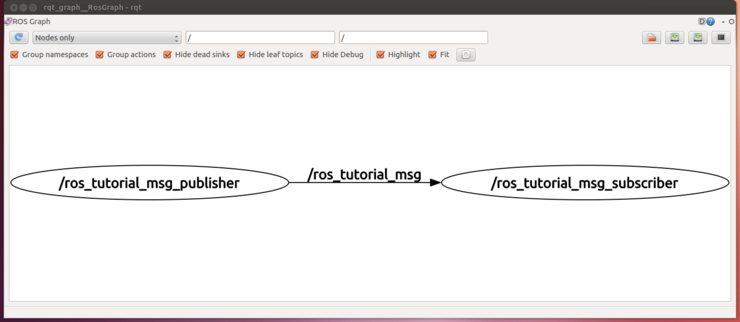
\includegraphics[width=\columnwidth]{pictures/chapter7/rqt_graph_oroca_ros_tutorials.png}
\caption{왼쪽: 서비스 서버 / 오른쪽: 서비스 클라이언트}
\end{figure}

※ 참고로, 서비스는 토픽과는 달리, 1회성이기에 ROS Graph 등에서 확인할 수 없다.

%-------------------------------------------------------------------------------
\subsection{서비스 콜 명령어 사용하는 방법 (rosservice call)}

서비스를 요청하는 방법으로는 위 9번 처럼 서비스 클라이언트 노드를 실행하는 방법도 있지만 "rosservice call" 이라는 명령어 및 rqt의 ServiceCaller 를 이용하는 방법이 있다. 그 중 우선, "rosservice call" 를 사용하는 방법에 대해서 알아보자.

\begin{lstlisting}[language=ROS]
$ rosservice call /ros_tutorial_srv 3 4
result: 7
\end{lstlisting}

위 처럼 "rosservice call" 명령어 뒤에 "/ros\_tutorial\_srv" 처럼 해당하는 서비스명을 적어주고 그 뒤를 이어 서비스 요청에 필요한 매개변수를 적어주면 된다. 위 예제에서는 아래와 같이 요청으로 int64 형태의 a 와 b 를 설정해 두었기때문에 매개변수로 "3"과 "4"를 입력해주었다. 이에 대한 서비스 응답의 결과값은 int64 형태의 sum이 7 이라고 돌아왔음을 확인 할 수 있다.  

\begin{lstlisting}[language=ROS]
int64 a
int64 b
---
int64 result
\end{lstlisting}

%-------------------------------------------------------------------------------
\subsection{GUI 툴인 ServiceCaller 를 사용하는 방법 (RQT ServiceCaller)}

마직막으로 gui 형태의 인터페이스를 이용한 rqt의 ServiceCaller 를 이용하는 방법이 있다. 우선, ROS의 GUI 툴인 rqt를 실행하자. 명령어는 아래와 같다.

\begin{lstlisting}[language=ROS]
$ rqt
\end{lstlisting}

그 뒤, 프로그램의 위 메뉴 중에 플러그인(Plugins)에서 ServiceCaller 를 선택하면 아래와 같은 화면이 나온다. 여기서 상단의 Service 에서 서비스명을 선택해주면 Request 에 서비스요청에 필요한 정보가 보인다. 서비스 요청을 해주기 위해서는 각 요청 정보의 Expressin에 정보를 기입해주면 된다. 필자는 a 란에 10, b란에 5를 입력하였다. 그 뒤, 오른쪽 상단의 녹색 전화기 모양의 Call 아이콘을 클릭해주면 서비스 요청이 실행되고, 화면 하단에 Response 란에 서비스 응답에 대한 결과가 표시된다. 위 10번에서 설명한 rosservice call 은 터미널에서 바로 실행이라는 장점이 있지만 리눅스 및 ROS 명령어 사용에 익숙하지 않은 사람에게는 ServiceCaller 를 추천한다.

\begin{figure}[h]
\centering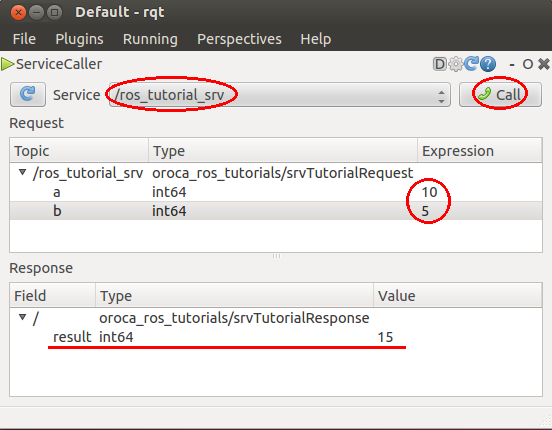
\includegraphics[width=0.7\columnwidth]{pictures/chapter7/rqt_service_caller.png}
\caption{ServiceCaller rqt플러그인을 통한 서비스 요청}
\end{figure}

강좌 15 및 16의 소스는 https://github.com/oroca/oroca\_ros\_tutorials 에서 확인해 볼 수 있다. 바로 적용해 보고 싶은 경우는 아래와 같이 catkin\_ws/src 에서 아래의 명령어를 실행해주면 된다.

\begin{lstlisting}[language=ROS]
$ cd ~/catkin_ws/src      %*(catkin/src 폴더로 이동*)
$ git clone https://github.com/oroca/oroca_ros_tutorials.git
$ cd ~/catkin_ws          %*(catkin 폴더로 이동*)
$ catkin_make             %*(catkin 빌드 실행*)
\end{lstlisting}

%-------------------------------------------------------------------------------
\section{매개변수 사용법}\index{매개변수 사용법}

%-------------------------------------------------------------------------------
\subsection{매개변수(parameter)}

\begin{definition*}[매개변수(parameter)]\label{def:RosParameter}
노드에서 사용되는 매개변수를 말한다. 흔히, 윈도우즈 프로그램에서 *.ini 설정파일과 같다고 생각하면 된다. 디폴트로 설정 값들이 지정되어 있고, 필요에 의해서 외부에서 이 매개변수를 읽기, 쓰기가 가능하다. 특히, 상황에 맞추어 이 매개변수를 외부에서 쓰기기능을 이용하여 설정값을 실시간으로 바꿀수 있기에 매우 유용한 방법이다. 예를들어 접속하는 USB포트 및 카메라 캘리브레이션 값, 속도 및 명령어들의 최대/최저 값 등의 설정등을 지정할 수 있다.
\end{definition*}

위의 매개변수는 강좌에서 여러번 언급되었으나 이번 강좌에서 처음으로 실습까지 다룰 것이다. 매개변수 개념과 관련된 좀 더 자세한 내용에 대해서 아래의 링크의 강좌를 참조하도록 하자. 특히, rosparam 명령어는 아래의 강좌를 통해서 이해했다는 전제하에 강좌를 진행하도록 하겠다.

%-------------------------------------------------------------------------------
\subsection{매개변수를 활용한 노드 작성}

이번 강좌에서는 이전 강좌 "로봇 운영체제 강좌 : 16. 서비스 서버 노드와 클라이언트 노드 작성 및 실행" 에서 다룬 "ros\_tutorial\_srv\_server.cpp" 의 소스를 수정하여 서비스 요청으로 입력된 "a" 와 "b" 를 단순히 덧셈하는 것이 아니라, 사칙연산을 할 수있도록 매개변수를 활용해 볼 것이다. 아래의 순서대로 이전 강좌에서 작성해둔 "ros\_tutorial\_srv\_server.cpp" 소스를 수정하도록 하자.

\begin{lstlisting}[language=ROS]
$ roscd oroca_ros_tutorials         %*(패키지 폴더로 이동한다.*)
$ cd src                            %*(노드의 소스코드 폴더인 src 폴더로 이동*)
$ gedit ros_tutorial_srv_server.cpp %*(소스 파일 신규 작성 및 내용 수정*)
\end{lstlisting}

\begin{lstlisting}[language=C++]
#include "ros/ros.h"                         //%* ROS 기본 헤더파일*)
#include "oroca_ros_tutorials/srvTutorial.h" //%* srvTutorial 서비스 파일 헤더*)
 
#define PLUS           1    //%* 덧셈*)
#define MINUS          2    //%* 빼기*)
#define MULTIPLICATION 3    //%* 곱하기*)
#define DIVISION       4    //%* 나누기*)
 
int g_operator = PLUS;
 
//%* 서비스 요청이 있을 경우, 아래의 처리를 수행한다*)
//%* 서비스 요청은 res, 서비스 응답은 req로 설정하였다*)
bool calculation(oroca_ros_tutorials::srvTutorial::Request  &req,
                 oroca_ros_tutorials::srvTutorial::Response &res)
{
  //%* 서비스 요청시 받은 a와 b 값을 파라미터값에 따라 연산자를 달리한다.*)
  //%* 계산한 후 서비스 응답값에 저장한다*)
  switch(g_operator){
    case PLUS:
         res.result = req.a + req.b; break;
    case MINUS:
         res.result = req.a - req.b; break;
    case MULTIPLICATION:
         res.result = req.a * req.b; break;  
    case DIVISION:
         if(req.b == 0){
           res.result = 0; break;
         }  
         else{
           res.result = req.a / req.b; break;  
         }
    default:
         res.result = req.a + req.b; break;
  }
 
  //%* 서비스 요청에 사용된 a, b값의 표시 및 서비스 응답에 해당되는 result 값을 출력한다*)
  ROS_INFO("request: x=%ld, y=%ld", (long int)req.a, (long int)req.b);
  ROS_INFO("sending back response: [%ld]", (long int)res.result);
 
  return true;
}
 
int main(int argc, char **argv)                     //%* 노드 메인 함수*)
{
  ros::init(argc, argv, "ros_tutorial_srv_server"); //%* 노드명 초기화*)
 
  ros::NodeHandle nh;                       //%* 노드 핸들 선언*)
 
  nh.setParam("calculation_method", PLUS);  //%* 매개변수 초기설정*)
 
  //%* 서비스 서버 선언, oroca\_ros\_tutorials 패키지의 srvTutorial 서비스 파일을 이용한*)
  //%* 서비스 서버 ros\_tutorial\_service\_server 를 작성한다. 서비스명은 "ros\_tutorial\_srv" 이며,*)
  //%* 서비스 요청이 있을경우, calculation 라는 함수를 실행하라는 설정이다*)
  ros::ServiceServer ros_tutorial_service_server =
    nh.advertiseService("ros_tutorial_srv", calculation);
 
  ROS_INFO("ready srv server!");
   
  ros::Rate r(10); //%* 10 hz*)
 
  while (1)
  {
    //%* 연산자를 매개변수로부터 받은 값으로 변경한다*)
    nh.getParam("calculation_method", g_operator);  
    ros::spinOnce();  //%* 콜백함수 처리루틴*)
    r.sleep();        //%* 루틴 반복을 위한 sleep 처리*)
  }
 
  return 0;
}
\end{lstlisting}

대부분은 이전 강좌에서 다룬 내용과 비슷하다. 이 중에서 매개변수 활용을 위해 추가된 부분에 대해서 알아보도록 하자. 특히, 49줄과 62줄에서 다룬 "setParam", "getParam" 가 매개변수 사용에서 제일 중요하다. 하지만, 매우 간단한 사용법이기때문에 함수 사용만 봐도 충분히 이해가 될 것이다.

%-------------------------------------------------------------------------------
\subsection{매개변수 설정}\index{매개변수 설정}

아래의 소스는 "calculation\_method" 라는 이름의 매개변수를 PLUS 라는 값으로 설정한다는 것이다. PLUS 는 위 소스에서 1 이므로 "calculation\_method" 매개변수는 1이 되고, 위 소스에서 서비스 요청으로 받은 값을 덧셈하여 서비스 응답을 하게 된다.

\begin{lstlisting}[language=C++]
nh.setParam("calculation_method", PLUS);
\end{lstlisting}

참로고 매개변수는 integers, floats, boolean, string, dictionaries, list 등으로 설정할 수 있다. 간단히 예를 들자면, 1 은 integer, 1.0은 floats, internetofthings은 string, true는 boolean, [1,2,3]은 integers 의 list, {a: b, c: d}은 dictionary이다. 

%-------------------------------------------------------------------------------
\subsection{매개변수 읽기}\index{매개변수 읽기}

아래의 소스는 "calculation\_method" 라는 이름의 매개변수를 불러와서 g\_operator 의 값으로 설정한다는 것이다. 이에 따라서 위 소스에서의 g\_operator 는 매 0.1초마다 매개변수의 값을 확인하여 서비스 요청으로 받은 값을 사칙연사중 어떤 계산을 하여 처리할 지 결정하게 된다.

\begin{lstlisting}[language=C++]
nh.getParam("calculation_method", g_operator);
\end{lstlisting}

%-------------------------------------------------------------------------------
\subsection{노드 빌드 및 실행}\index{노드 빌드 및 실행}

\begin{lstlisting}[language=ROS]
$ cd ~/catkin_ws && catkin_make
\end{lstlisting}

위의 명령어로 oroca\_ros\_tutorials 패키지의 서비스 서버 노드가 빌드되었다. 

\begin{lstlisting}[language=ROS]
$ rosrun oroca_ros_tutorials ros_tutorial_srv_server 
[ INFO] [1385278089.933322980]: ready srv server!
\end{lstlisting}

위 명령어를 실행하면 서비스 서버는 서비스 요청 대기를 하게 된다.

%-------------------------------------------------------------------------------
\subsection{매개변수 리스트 보기}\index{매개변수 리스트 보기}

\begin{lstlisting}[language=ROS]
$ rosparam list
/calculation_method
/rosdistro
/roslaunch/uris/host_192_168_4_185__60432
/rosversion
/run_id
\end{lstlisting}

"rosparam list" 명령어로 현재 ROS 네트워크에 사용된 매개변수의 목록을 확인할 수 있다. 위에 출력된 목록중 "/calculation\_method" 가 우리가 사용한 매개변수이다.

%-------------------------------------------------------------------------------
\subsection{매개변수 사용예}\index{매개변수 사용예}

아래의 명령어 대로 매개변수를 설정해보고, 매번 같은 서비스 요청을 하여 서비스 처리가 달라짐을 확인해보자.

\begin{lstlisting}[language=ROS]
$ rosservice call /ros_tutorial_srv 10 5
result: 15
$ rosparam set /calculation_method 2
$ rosservice call /ros_tutorial_srv 10 5
result: 5
$ rosparam set /calculation_method 3
$ rosservice call /ros_tutorial_srv 10 5
result: 50
$ rosparam set /calculation_method 4
$ rosservice call /ros_tutorial_srv 10 5
result: 2 
\end{lstlisting}

"rosparam set" 명령어로 "calculation\_method" 매개변수를 바꿀 수 있다. 바뀐 매개변수로 매번 같은 입력인 "rosservice call /ros\_tutorial\_srv 10 5"을 했음에도 불구하고 결과값이 각가 다른것을 확인할 수 있다.  이처럼 ROS에서 매개변수는 노드 외부로부터 노드의 흐름 및 설정, 처리 등을을 바꿀 수 있다. 매우 유용한 기능이기에 지금 당장 쓰지 않더라도 꼭 알아두도록 하자.


%-------------------------------------------------------------------------------
\section{로스런치 사용법}\index{로스런치 사용법}

%-------------------------------------------------------------------------------
\subsection{로스런치}\index{로스런치}

\begin{definition}[roslaunch]
로스런(rosrun)이 하나의 노드를 실행하는 명령어라면 로스런치(roslaunch\footnote{ROS Wiki roslaunch, http://wiki.ros.org/roslaunch})는 복 수개의 노드를 실행하는 개념이다. 이 명령어를 통해 정해진 단일 혹은 복수의 노드를 실행시킬 수 있다. 

그 이외의 기능으로 실행시에 패키지의 매개변수를 변경, 노드 명의 변경, 노드 네임 스페이스 설정, ROS\_ROOT 및 ROS\_PACKAGE\_PATH 설정, 이름 변경, 환경 변수 변경 등의 실행시 변경할 수 있는 많은 옵션들을 갖춘 노드 실행에 특화된 로스 명령어이다. 

로스런치는 "*.launch" 라는 로스런치파일을 사용하여 실행 노드에 대한 설정을 해주는데 이는 XML 기반으로 되어 있으며, 태그별 옵션을 제공하고 있다. 실행 명령어로는 "roslaunch 패키지명 로스런치파일" 이다.
\end{definition}

%-------------------------------------------------------------------------------
\subsection{로스런치의 활용}\index{로스런치의 활용}

로스런치의 활용으로 이전 강좌인 "로봇 운영체제 강좌 : 15. 메시지 발행자 노드와 구독자 노드 작성 및 실행" 에서 작성한 ros\_tutorial\_msg\_publisher 와  ros\_tutorial\_msg\_subscriber 를 이름을 바꾸어서 실행해보자. 그냥 이름을 바꾸어 의미가 없으니, 발신자 노드와 구독자 노드를 각각 두 개씩 구동하여 서로간에 별도로 메시지 통신을 해보도록 하겠다.

우선, *.launch 파일을 작성하자. 로스런치 파일은 *.launch 이라는 파일명을 가지고 있으며, 노드 폴더에 로스런치를 저장할 launch 라는 폴더를 생성해줘야 한다. 아래의 명령어대로 폴더를 생성하고 새롭게 union.launch 이라는 파일으로 로스런치 파일을 생성해보자.

\begin{lstlisting}[language=ROS]
$ cd ~/catkin_ws/src/oroca_ros_tutorials
$ mkdir launch
$ cd launch
$ gedit union.launch
\end{lstlisting}

내용으로는 아래의 내용대로 작성해주도록 하자.

\begin{lstlisting}[language=XML]
<launch>
  <node pkg="oroca_ros_tutorials" type="ros_tutorial_msg_publisher"   name="msg_publisher1"/>
  <node pkg="oroca_ros_tutorials" type="ros_tutorial_msg_subscriber"  name="msg_subscriber1"/>

  <node pkg="oroca_ros_tutorials" type="ros_tutorial_msg_publisher"  name="msg_publisher2"/>
  <node pkg="oroca_ros_tutorials" type="ros_tutorial_msg_subscriber"  name="msg_subscriber2"/>
</launch>
\end{lstlisting}

\begin{description}
\item[\textless launch\textgreater] 는 로스런치 태그로써 이 태그안에는 로스런치에 필요한 태그들이 기술된다.
\item[\textless node\textgreater] 는 로스런치로 실행할 노드를 기술하게 된다. 옵션으로는 pkg, type, name 이 있다. pkg는 패키지의 이름, type는 실제 실행할 노드의 이름, name은 type를 실행하되 실행할때 붙여지는 이름이다.  
\end{description}

로스런치파일의 작성을 마쳤으면 아래와 같이 로스런치를 실행해주자.

\begin{lstlisting}[language=ROS]
$ roslaunch oroca_ros_tutorials union.launch
\end{lstlisting}

실행 후, 결과가 어떻게 되었을까? 우선 아래와 같이 "rosnode list" 명령어로 현재 실행중인 노드를 살펴보자. 결과적으로  ros\_tutorial\_msg\_publisher 노드가 msg\_publisher1 및 msg\_publisher2 로 이름이 바뀌어 두 개의 노드가 실행되었으며, ros\_tutorial\_msg\_subscriber 노드도  msg\_subscriber1 및 msg\_subscriber2 로 이름이 바뀌어 실행되었다.  

\begin{lstlisting}[language=ROS]
$ rosnode list
/msg_publisher1
/msg_publisher2
/msg_subscriber1
/msg_subscriber2
/rosout
\end{lstlisting}

문제는,"발신자 노드와 구독자 노드를 각각 두 개씩 구동하여 서로간에 별도로 메시지 통신" 하게한다는 첫 의도와는 다르게 rqt\_graph 를 통해 보면 서로간의 메시지를 모두 구독하고 있다는 것이다. 이는 단순히 실행되는 노드의 이름만을 변경해 주었을뿐 사용되는 메시지의 이름을 바꿔주지 않았기 때문이다. 이 문제를 다른 로스런치 태그를 사용하여 해결해보자.

\begin{figure}[h]
\centering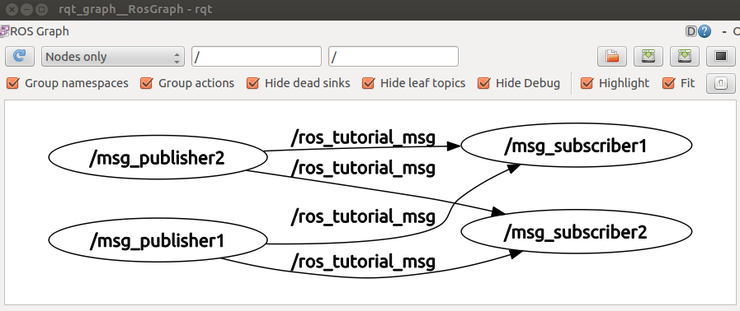
\includegraphics[width=0.9\columnwidth]{pictures/chapter7/rqt_graph_oroca_ros_tutorials_union1.png}
\caption{roslaunch를 이용하여 복수개의 노드를 실행하였을 때의 모습}
\end{figure}

\begin{lstlisting}[language=ROS]
$ rqt_graph
\end{lstlisting}

미리 만들어둔 union.launch 을 수정해보자.

\begin{lstlisting}[language=ROS]
$ cd ~/catkin_ws/src/oroca_ros_tutorials/launch
$ gedit union.launch
\end{lstlisting}

내용으로는 아래의 내용대로 작성해주도록 하자.

\begin{lstlisting}[language=XML]
<launch>

  <group ns="ns1">
    <node pkg="oroca_ros_tutorials" type="ros_tutorial_msg_publisher"   name="msg_publisher"/>
    <node pkg="oroca_ros_tutorials" type="ros_tutorial_msg_subscriber"  name="msg_subscriber"/>
  </group>

  <group ns="ns2">
    <node pkg="oroca_ros_tutorials" type="ros_tutorial_msg_publisher"  name="msg_publisher"/>
    <node pkg="oroca_ros_tutorials" type="ros_tutorial_msg_subscriber"  name="msg_subscriber"/>
  </group>

</launch>
\end{lstlisting}

\textbf{\textless group\textgreater} 는 지정된 노드를 그룹으로 묶어주는 태그이다. 옵션으로는 ns 가 있다. 이는 네임스페이스(namespace)로써 그룹의 이름을 지칭하며, 그룹에 속한 노드의 이름 및 메시지 등도 모두 ns로 지정한 이름에 포함되게 된다.


다시 한번, rqt\_graph 로 노드간의 연결 및 메시지 송수신 상태를 확인해보자. 이번에는 우리가 처음에 의도한 "발신자 노드와 구독자 노드를 각각 두 개씩 구동하여 서로간에 별도로 메시지 통신" 가 성공적으로 이루어졌음을 확인할 수 있다.

\begin{lstlisting}[language=ROS]
$ rqt_graph
\end{lstlisting}

\begin{figure}[h]
\centering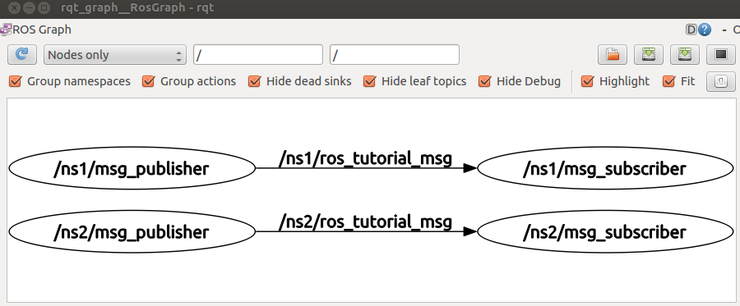
\includegraphics[width=0.9\columnwidth]{pictures/chapter7/rqt_graph_oroca_ros_tutorials_union2.png}
\caption{네임스페이스를 이용하였을 때의 메시지 통신}
\end{figure}

%-------------------------------------------------------------------------------
\subsection{로스런치에 사용되는 태그}

로스런치는 로스런치 파일에서 XML\footnote{ROS Wiki roslaunch XML,  http://wiki.ros.org/roslaunch/XML}을 어떻게 작성하냐에 따라 다양한 응용이 가능할 것이다. 현재 로스런치에서 사용되는 태그들은 아래와 같다. 많이 사용되는 태그는 위에서 설명했고 그 이외에 필요한 부분에 대해서는 직접 찾아가보며 익혀보도록 하자. 각 태그에 링크로 설명 페이지의 주소를 걸어두었으니 필요한 태그의 공식 설명을 참조해보길 바란다.

\begin{description}
\item[\textless launch\textgreater] 로스런치 구문의 시작과 끝을 가르킨다.
\item[\textless node\textgreater] 노드 실행에 대한 태그이다. 패키지, 노드명, 실행명을 변경할 수 있다.
\item[\textless machine\textgreater] 노드를 실행하는 PC의 이름, address,  ros-root,  ros-package-path 등을 설정할 수 있다.
\item[\textless include\textgreater] 다른 패키지 및 같은 패키지에 속해있는 다른 로스런치를 불러와 하나의 파일처럼 실행 시킬 수 있다.
\item[\textless remap\textgreater] 토픽 이름 등의 노드에서 사용중인 로스변수의 이름을 변경할 수 있다. 
\item[\textless env\textgreater] 환경 변수를 변경한다.
\item[\textless param\textgreater] 로스 매개변수를 변경한다
\item[\textless rosparam\textgreater] 로스런치에서 rosparam 의 명령어를 이용하는 태그이다.
\item[\textless group\textgreater] 실행되는 노드를 그룹화할때 사용되는 태그이다.
\item[\textless test\textgreater] 노드를 테스트할 때 사용되는 태그로 \textless node\textgreater 와 비슷하지만 테스트에 사용되는 옵션들이 추가되어 있다.
\item[\textless arg\textgreater] 로스런치에서 사용되는 변수를 정의할 수 있고, 로스런치에서 변수처럼 재사용되어 주소 및 대체 이름등에 사용된다.
\end{description}

%-------------------------------------------------------------------------------